\documentclass[final]{beamer}

% ====================
% Packages
% ====================

\usepackage[T1]{fontenc}
\usepackage{lmodern}
\usepackage[orientation=portrait,size=a0,scale=1.6]{beamerposter}
\usetheme{gemini}
\usecolortheme{unibz}
\usepackage{dl}
\usepackage{bookmark}
\usepackage{graphicx}
\usepackage{booktabs}
\usepackage{tikz}
\usepackage{pgfplots}
\usepackage{amsmath}
\usepackage{amssymb}
\usepackage{mathtools}
\usepackage{algorithm}
\usepackage{algpseudocode}
\usepackage{adjustbox}
\usepackage{xspace}
\usepackage{url}
\pgfplotsset{compat=1.14}
\usepackage{anyfontsize}
\usepackage[numbers]{natbib}

\AtBeginDocument{\bibsep=0pt}
\bibliographystyle{elsarticle-num-names}

% ====================
% Lengths
% ====================

\newlength{\sepwidth}
\newlength{\colwidth}
\setlength{\sepwidth}{0.025\paperwidth}
\setlength{\colwidth}{0.45\paperwidth}

\newcommand{\separatorcolumn}{\begin{column}{\sepwidth}\end{column}}
% theorems and the like
% \newtheorem{theorem}{Theorem}
\newtheorem{lemma}{Lemma}
% \newtheorem{proposition}{Proposition}
% \newtheorem{corollary}{Corollary}

% \theorembodyfont{\rmfamily}
% \newtheorem{definition}{Definition}
% \newtheorem{example}{Example}

% \theorembodyfont{\slshape}
% \newtheorem{assumption}{Assumption}

% \theorembodyfont{\slshape}
% \newtheorem{hypothesis}{Hypothesis}

% \newenvironment{justification}{\textsf{Justification:}}{\hfill $\Box$}
%\newenvironment{proof}{\noindent\textsc{proof:}}{\hfill $\square$ \bigskip}


\newcommand{\AL}{\ensuremath{\mathcal{AL}}\xspace}
\newcommand{\ALC}{\ensuremath{\mathcal{ALC}}\xspace}
\newcommand{\SROIQ}{\ensuremath{\mathcal{SROIQ}}\xspace}
\newcommand{\onto}[1]{\ensuremath{\mathsf{#1}}}
\usepackage[colorinlistoftodos]{todonotes}

\newcommand{\cg}
{\ensuremath{\blacktriangle}\xspace}
%{\ensuremath{\dot{\sqcup}}\xspace}

\newcommand{\todoT}[1]{\todo[fancyline,size=\small,color=orange!40]{\textbf{TBD:} #1}\xspace}
\newcommand{\todoR}[1]{\todo[fancyline,size=\small,color=orange!40]{\textbf{rc:} #1}\xspace}

\newcommand{\todoO}[1]{\todo[fancyline,size=\small,color=red!20]{\textbf{ok:} #1}\xspace}

\newcommand{\tododo}[1]{\todo[fancyline,size=\small,color=red!60]{\textbf{ToDO:} #1}\xspace}
\newcommand{\todoin}[1]{\todo[inline,size=\small,color=green!20]{\textbf{HERE:} #1}\xspace}


%\usepackage{pgf}https://preview.overleaf.com/public/pqghhhhwjqpw/images/986e3685291cb332a5fbe5a979b5045d2e649a43.jpeg
\usepackage{tikz}
%\usetikzlibrary{arrows,automata}
\usetikzlibrary{positioning,calc,backgrounds}

%%%%%%%MACROS%%%%%%%%
\newcommand{\Imc}{\ensuremath{\mathcal{I}}\xspace}
\newcommand{\Jmc}{\ensuremath{\mathcal{J}}\xspace}
\newcommand{\Tmc}{\ensuremath{\mathcal{T}}\xspace}
\newcommand{\Amc}{\ensuremath{\mathcal{A}}\xspace}
\newcommand{\Rmc}{\ensuremath{\mathcal{R}}\xspace}
\newcommand{\Omc}{\ensuremath{\mathcal{O}}\xspace}
\newcommand{\Omcref}{\ensuremath{\mathcal{O}_\mathrm{ref}}\xspace}
\newcommand{\Omcfull}{\ensuremath{\mathcal{O}_\mathrm{full}}\xspace}
\newcommand{\Ontology}{\Omc}

% \newcommand{\sub}{\ensuremath{\mathsf{sub}}\xspace}
\newcommand{\subr}{\ensuremath{\mathsf{subr}}\xspace}

\newcommand{\EL}{\ensuremath{\mathcal{E\!L}}\xspace}
\newcommand{\elpp}{\ensuremath{\mathcal{E\!L}^{++}}\xspace}
% \newcommand{\DL}{{\ensuremath{\mathcal{DL}}}\xspace}

\newcommand{\Inf}{{\ensuremath{\mathsf{Inf}}}\xspace}
\newcommand{\qual}{{\ensuremath{\mathsf{IIC}}}\xspace}

\newcommand{\Tup}{{\ensuremath{\mathsf{UpCover}_\Ontology}}\xspace}
\newcommand{\Tdown}{{\ensuremath{\mathsf{DownCover}_\Ontology}}\xspace}
\newcommand{\gammaT}{{\ensuremath{\gamma_\mathcal{T}}}\xspace}
\newcommand{\rhoT}{{\ensuremath{\rho_\mathcal{T}}}\xspace}
%\newcommand{\gammaT}{{\ensuremath{\gamma_{\mathcal{T}}}\xspace}
%\newcommand{\rhoT}{{\ensuremath{\rho_{\mathcal{T}}}\xspace}

\newcommand{\disjoint}{\ensuremath{\mathit{disjoint}}\xspace}
\newcommand{\self}{\ensuremath{\mathit{Self}}\xspace}
\newcommand{\less}[2]{\ensuremath{\leq #1~#2}\xspace}
\newcommand{\more}[2]{\ensuremath{\geq #1~#2}\xspace}
\newcommand{\nominal}[1]{\ensuremath{\{#1\}}\xspace}

\newcommand{\inv}{\ensuremath{\mathit{inv}}\xspace}
\newcommand{\refine}{\ensuremath{\mathop{\uparrow}}\xspace}
\newcommand{\corefine}{\ensuremath{\mathop{\downarrow}}\xspace}
%\DeclareMathOperator*{\argmax}{\mathsf{arg\,max}}
\DeclareMathOperator*{\argmax}{\mathsf{argmax}}


% ====================
% Title
% ====================

\title{Making Axiom Weakening Work in \bfSROIQ}
\author{Roland Bernard \and Oliver Kutz \and Nicolas Troquard}
\institute[shortinst]{Free University of Bozen-Bolzano}

% ====================
% Logo
% ====================

\logoright{
\includegraphics[height=7cm]{unibz-logo.pdf}}

% ====================
% Body
% ====================

\begin{document}

\begin{frame}[t]
  
\begin{columns}[t]
\separatorcolumn

\begin{column}{\colwidth}
  \begin{block}{Introduction}
    \textbf{Background} \vskip-.5ex
    \begin{itemize}
      \item Many methods for fixing inconsistent ontologies involve identifying and removing problematic axioms.
      \item This approach can lead to unnecessary information loss.
      \item Axiom weakening is a more information preserving approach and has previously been explored for \ALC.
    \end{itemize}

    \textbf{In this paper} \vskip-.5ex
    \begin{itemize}
      \item We extend axiom weakening principles to \SROIQ, including weakening of RIAs.
      \item We discuss a number of scenarios where weakening can impact regularity of \SROIQ RBoxes, and provide a framework where this is avoided.
      \item We perform experimental evaluation of repairing \SROIQ ontologies with axiom weakening.
    \end{itemize}
  \end{block}
\end{column}

\separatorcolumn

\begin{column}{\colwidth}
  \begin{block}{Axiom Weakening for Ontology Repair}
    To achieve axiom weakening, two types of refinement operators are used, a specialization operator and a generalization operator. These are used to define the axiom weakening operator. These operators need a consistent reference ontology to yield useful results. The process for repairing an inconsistent ontology proceeds as follows:

    \textbf{Repairing ontologies} \vskip-.5ex
    \begin{enumerate}
      \item Choose a consistent subset as the reference ontology.
      \item Select a problematic axiom.
      \item Weaken the selected axiom using the axiom weakening operator.
      \item Replace the selected axiom with the weaker axiom.
      \item Repeat steps 2-4 until the ontology is consistent. 
    \end{enumerate}
  \end{block}
\end{column}

\separatorcolumn
\end{columns}

\begin{columns}[t]
\separatorcolumn

\begin{column}{2\colwidth+\sepwidth}
  \begin{block}{Extending Axiom Weakening to \bfSROIQ}

  \begin{minipage}[t]{0.5\linewidth-1ex}
    \textbf{Difficulties} \vskip-.5ex
    \begin{itemize}
      \item \SROIQ imposes global restrictions on the ontology that can not be checked by looking at axiom separately.
      \item Non-simple roles may not be used in cardinality constraints, \self constraints, or disjoint role axioms.
      \item RBoxes must be regular.
      \item[\raisebox{.2ex}{\lapbox[\width]{.5ex}{$\Rightarrow$}}] Adding valid axioms (e.g., weakenings) to a valid \SROIQ ontology can make the ontology invalid.
    \end{itemize}

    \begin{exampleblock}{\normalsize Example: Weakening that breaks regularity}
      Take the ontology
      \begin{align*}
        \Omc &= \{ r \circ s \circ r \sqsubseteq t, \top \sqsubseteq \forall t.\nominal a, \top \sqsubseteq \exists s.\nominal a \} \enspace .
      \end{align*}
      Since the range of $t$ is restricted to the single individual $a$, and $s$ contains all connections to $a$, $t \sqsubseteq_\Omc s$. The axiom $r \circ s \circ r \sqsubseteq t$ could therefore be weakened to $r \circ s \circ r \sqsubseteq s$. Yet, this would result in a non-regular RBox.
    \end{exampleblock}
  \end{minipage}
  \hspace{1ex}
  \begin{minipage}[t]{0.5\linewidth-1ex}
    \textbf{Avoiding these problems} \vskip-.5ex
    \begin{itemize}
      \item The allowed weakenings must be restricted to ensure the result is a \SROIQ ontology.
      \item We only use simple roles whenever we have to replace roles using the refinement operators.
      \item For RIAs we only ever refine the super role if the RIA is simple and the sub role is simple.
      \item[\raisebox{.2ex}{\lapbox[\width]{.5ex}{$\Rightarrow$}}] These two rule ensure that all simple roles remain simple even after applying the weakening.
      \item[\raisebox{.2ex}{\lapbox[\width]{.5ex}{$\Rightarrow$}}] They further guarantee that the RBox remains regular.
    \end{itemize}

    \begin{alertblock}{\normalsize Theorem}
      Given that the original ontology to be repair and the reference ontology are valid \SROIQ ontologies. For every axiom $\phi$ of the original ontology, if $\phi'$ is a weakening of $\phi$ generated using the weakening operator, then the result of adding $\phi'$ to the original ontology is also a valid \SROIQ ontology.
    \end{alertblock}
  \end{minipage}

  \end{block}
\end{column}

\separatorcolumn
\end{columns}

\begin{columns}[t]
\separatorcolumn

\begin{column}{\colwidth}
  \begin{block}{Experimental Evaluation}
    \textbf{Performed experiment} \vskip-.5ex
    \begin{enumerate}
      \item Selected different ontologies from BioPortal.
      \item Generated inconsistent ontologies by adding axioms.
      \item Repaired the inconsistent ontologies using both removal and axiom weakening.
      \item Compared the quality of the resulting repairs using \qual.
    \end{enumerate}
    \vskip-1ex
    \begin{figure}
      \begin{adjustwidth}{-2ex}{0ex}
        \centering
        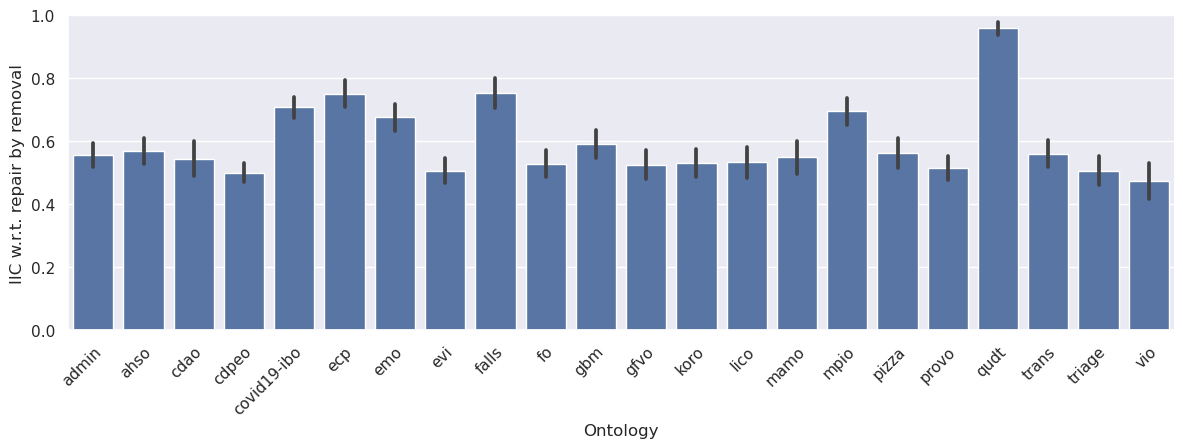
\includegraphics[width=\textwidth+2ex]{figures/iic-remove-ontology-bar.png}
      \end{adjustwidth}
      \caption{Mean IIC with respect to repair via removal per ontology. The error bars show the 95\% confidence interval.}
      \label{fig:results-remove}
    \end{figure}
  \end{block}
\end{column}

\separatorcolumn

\begin{column}{\colwidth}
  \begin{block}{Conclutions and Outlook}
    \textbf{Conclusions} \vskip-.5ex
    \begin{itemize}
      \item Selected different ontologies from BioPortal.
      \item Generate inconsistent ontologies by adding axioms.
      \item Repaired the inconsistent ontologies using both removal and axiom weakening.
      \item Compare the quality of the resulting repairs using \qual.
    \end{itemize}

    \textbf{Outlook} \vskip-.5ex
    \begin{itemize}
      \item Selected different ontologies from BioPortal.
      \item Generate inconsistent ontologies by adding axioms.
      \item Repaired the inconsistent ontologies using both removal and axiom weakening.
      \item Compare the quality of the resulting repairs using \qual.
    \end{itemize}
  \end{block}
\end{column}

\separatorcolumn
\end{columns}

% \vfill

% \footnotesize{\bibliography{biblio}}

\end{frame}

\end{document}
